\begin{longtable}{|p{0.2\textwidth}|p{0.2\textwidth}|p{0.2\textwidth}|p{0.25\textwidth}|p{0.1\textwidth}|}
    \caption{Usability Test Cases} \\
    \hline
    \textbf{Test Case ID} & \textbf{Objective} & \textbf{Test Steps} & \textbf{Expected Results} & \textbf{Status} \\
    \hline
    \endfirsthead
    \multicolumn{5}{c}%
    {{\bfseries \tablename\ \thetable{} -- continued from previous page}} \\
    \hline
    \textbf{Test Case ID} & \textbf{Objective} & \textbf{Test Steps} & \textbf{Expected Results} & \textbf{Status} \\
    \hline
    \endhead
    \hline \multicolumn{5}{|r|}{{Continued on next page}} \\ \hline
    \endfoot
    \hline
    \endlastfoot

    % General Usability
    TC-USAB-001 & Verify the clarity and intuitiveness of the login page. & 1. Navigate to the login page. \newline 2. Observe the layout and labels. \newline 3. Attempt to log in with incorrect credentials. & 1. The page is uncluttered with clear input fields for "Email" and "Password". \newline 2. A clear, non-technical error message is displayed upon failed login. \newline 3. The purpose of the page is immediately understandable. & To Be Executed \\
    \hline
    TC-USAB-002 & Assess the consistency of the main navigation menu across different pages. & 1. Log in as a Librarian. \newline 2. Navigate to Dashboard, Users, Books, and Authors pages. \newline 3. Observe the position, style, and icons of the navigation sidebar. & The navigation sidebar remains in a consistent location and maintains the same look and feel across all pages. The active page is clearly highlighted. & To Be Executed \\
    \hline
    TC-USAB-003 & Evaluate the effectiveness of user feedback for common actions. & 1. Log in as a Librarian. \newline 2. Create a new Author. \newline 3. Update the details of an existing Book. \newline 4. Delete a Genre. & 1. A clear success message (e.g., a toast or snackbar) appears after each successful action. \newline 2. A confirmation dialog appears before the deletion, preventing accidental data loss. \newline 3. Feedback is timely and easy to understand. & To Be Executed \\
    \hline

    % Librarian Specific
    TC-USAB-004 & Evaluate the clarity and usefulness of the Librarian's dashboard. & 1. Log in as a Librarian. \newline 2. View the dashboard. \newline 3. Analyze the widgets for "Total Books", "Total Members", etc. \newline 4. Review the charts. & 1. The dashboard provides a clear, at-a-glance summary of key library statistics. \newline 2. Charts are well-labeled and easy to interpret. \newline 3. The visual hierarchy directs attention to important information. See Figure \ref{fig:dashboard_usability}. & To Be Executed \\
    \hline
    TC-USAB-005 & Test the ease of creating a new user. & 1. Navigate to the "User" page. \newline 2. Click the "New User" button. \newline 3. Fill out the user creation form with valid data. \newline 4. Submit the form. & The process is intuitive. Form fields are clearly labeled, and input requirements (e.g., password complexity) are clear. The new user appears in the user list immediately after creation. & To Be Executed \\
    \hline
    TC-USAB-006 & Test the intuitiveness of the book management workflow. & 1. Navigate to the "Book" page. \newline 2. Use the filter/search bar to find a specific book. \newline 3. Click to edit a book. \newline 4. Change the book's genre and save. & The search functionality is easy to find and use. Editing a book is straightforward, with a clear form and save button. The UI updates instantly to reflect the change. & To Be Executed \\
    \hline

    % Member Specific
    TC-USAB-007 & Evaluate the process of borrowing a book for a Member. & 1. Log in as a Member. \newline 2. Find an available book. \newline 3. Click the "Borrow" button. \newline 4. Confirm the action. & The "Borrow" action is clearly available for books that are not already on loan. The process requires minimal steps. The user receives clear confirmation that the book has been successfully borrowed. & To Be Executed \\
    \hline
    TC-USAB-008 & Assess the clarity of the member's borrowal history page. & 1. Log in as a Member. \newline 2. Navigate to the "Borrowals" page. \newline 3. View the list of current and past borrowals. & The page clearly displays essential information: book title, borrow date, due date, and status (e.g., "Borrowed", "Returned"). The layout is easy to read and understand. See Figure \ref{fig:borrowal_history_usability}. & To Be Executed \\
    \hline
    TC-USAB-009 & Test the ease of leaving a review for a book. & 1. Log in as a Member. \newline 2. Navigate to a book they have borrowed. \newline 3. Find the option to leave a review. \newline 4. Submit a rating and a comment. & The review submission form is easy to find and use. The user can easily select a rating (e.g., via stars) and type a comment. The submitted review appears promptly. & To Be Executed \\
    \hline

\end{longtable}

\begin{figure}[H]
    \centering
    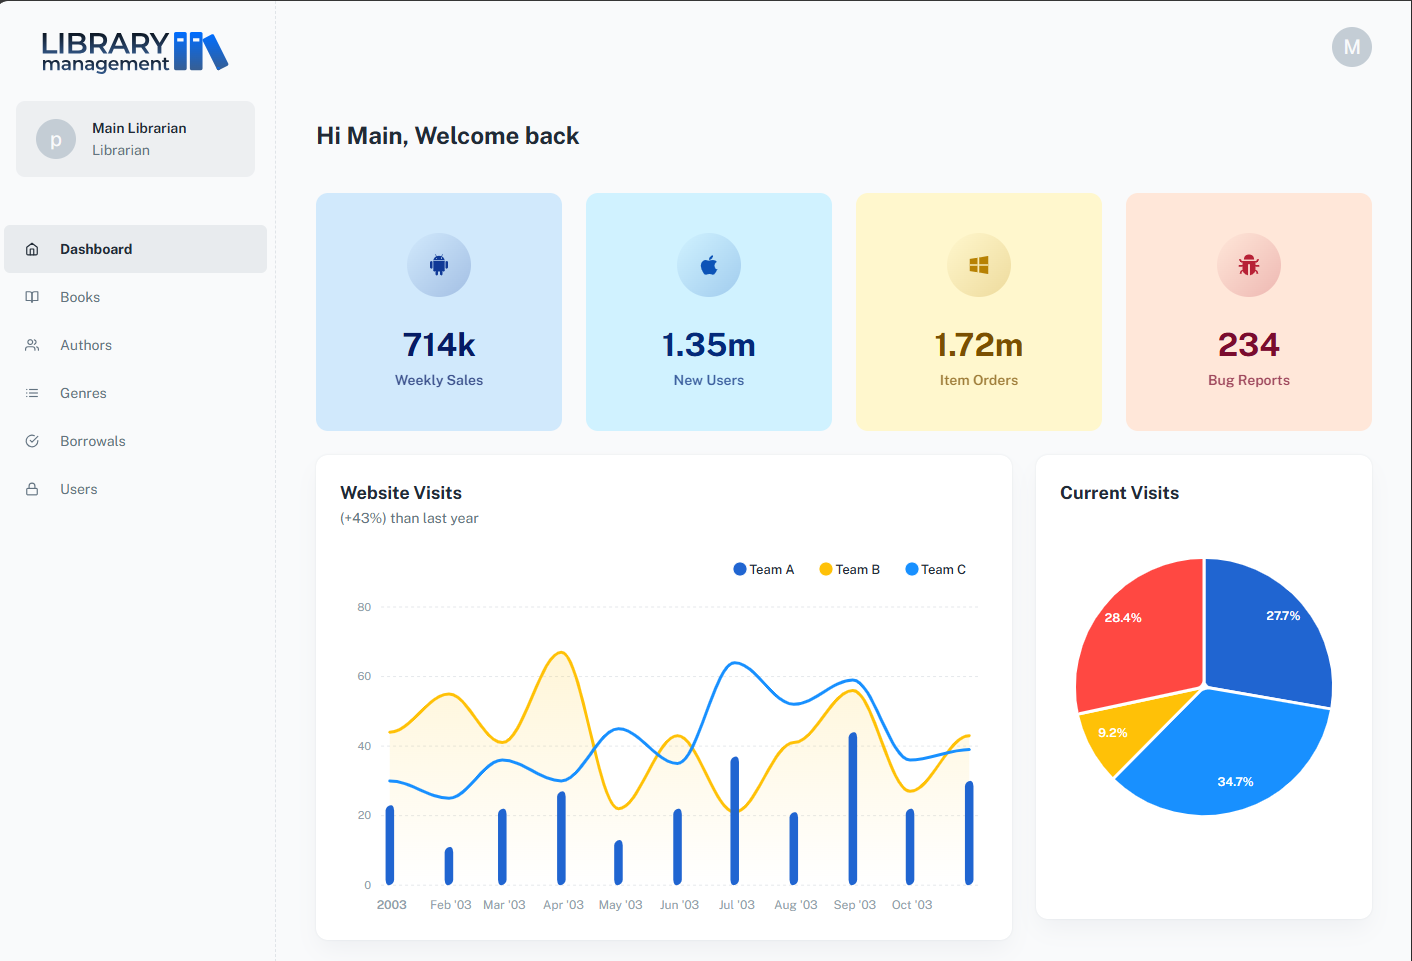
\includegraphics[width=0.9\textwidth]{assets/dashboard_screenshot.png}
    \caption{Librarian Dashboard UI for Usability Evaluation}
    \label{fig:dashboard_usability}
\end{figure}

\begin{figure}[H]
    \centering
    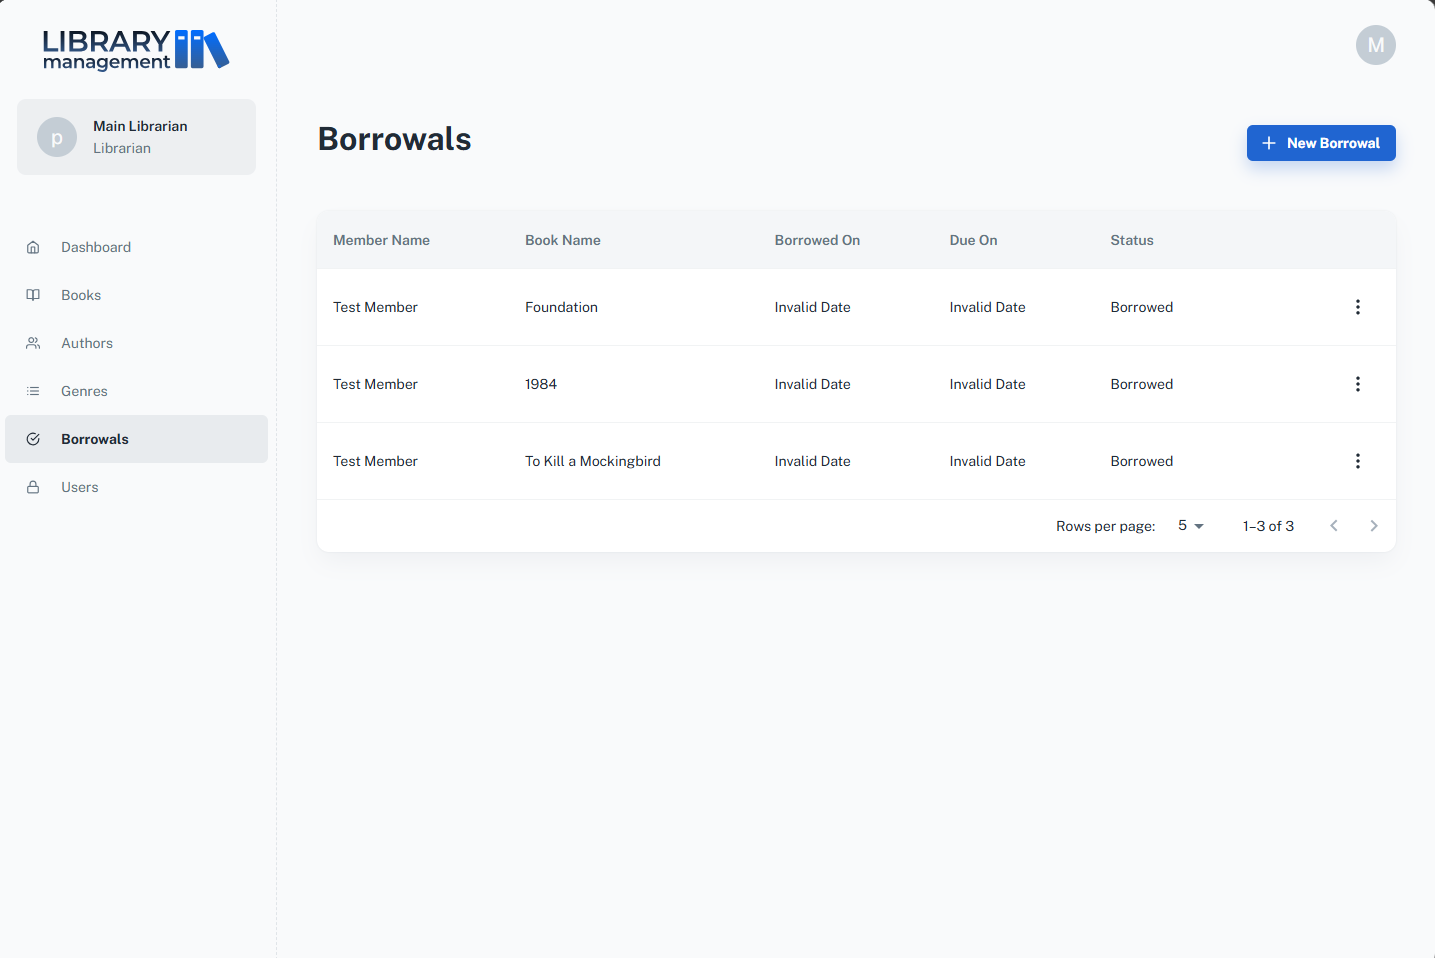
\includegraphics[width=0.9\textwidth]{assets/borrowal_history_member.png}
    \caption{Member Borrowal History UI for Usability Evaluation}
    \label{fig:borrowal_history_usability}
\end{figure}